
% ------------------------------------------------------------------------
\chapter{Simulator Structure}

\begin{refsection}



LinkPlanner is a signals open-source simulator.

The major entity is the system.

A system comprises a set of blocks.

The blocks interact with each other through signals.

\section{System}

\section{Blocks}

\section{Signals}

List of available signals:

\begin{itemize}
    \item Signal

\end{itemize}

\subsubsection{PhotonStreamXY}
A single photon is described by two amplitudes $A_x$ and $A_y$ and a phase difference between them, $\delta$. This way, the signal PhotonStreamXY is a structure with two complex numbers, $x$ and $y$.


\subsubsection{PhotonStreamXY\_MP}
The multi-path signals are used to simulate the propagation of a quantum signal when the signal can follow multiple paths. The signal has information about all possible paths, and a measurement performed in one path immediately affects all other possible paths.
From a Quantum approach, when a single photon with a certain polarization angle reaches a $50:50$ Polarizer, it has a certain probability of follow one path or another. In order to simulate this, we have to use a signal PhotonStreamXY\_MP, which contains information about all the paths available. In this case, we have two possible paths: $0$ related with horizontal and $1$ related with vertical. This signal is the same in both outputs of the polarizer. The first decision is made by the detector placed on horizontal axis. Depending on that decision, the information about the other path $1$ is changed according to the result of the path $0$. This way, we guarantee the randomness of the process. So, signal PhotonStreamXY\_MP is a structure of two PhotonStreamXY indexed by its path.


\section{Log File}
\subsection{Introduction}
The Log File allows for a detailed analysis of a simulation. It will output a file containing the timestamp when a block is initialized, the number of samples in the buffer ready to be processed for each input signal, the signal buffer space for each output signal and the amount of time in seconds that took to run each block. Log File is enabled by default, so no change is required. If you want to turn it off, you must call the set method for the logValue and pass $false$ as argument. This must be done before method $run()$ is called, as shown in line 125 of Figure \ref{fig:logfileexample}.

\renewcommand{\figurename}{Figure}
\begin{figure}[H]
\centering
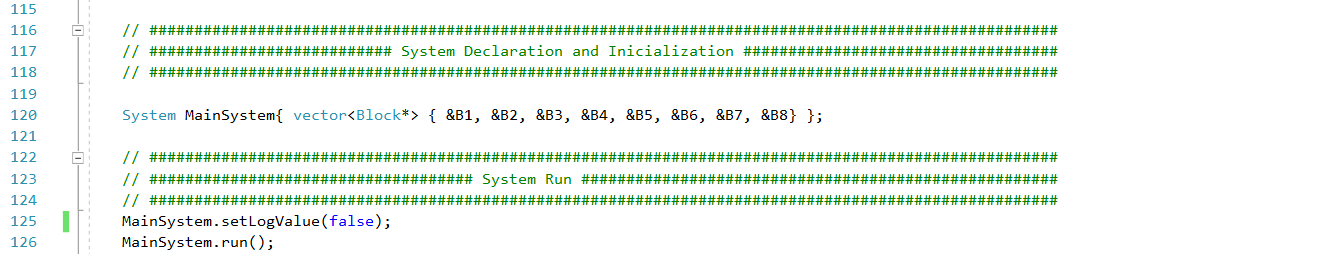
\includegraphics[width=1.3\linewidth]{./chapter/simulator_structure/figures/log_file_example}
\caption{Disabling Log File}
\label{fig:logfileexample}
\end{figure}

\subsection{Parameters}
The Log File accepts two parameters: $logFileName$ which correspond to the name of the output file, i.e., the file that will contain all the information listed above and $logValue$ which will enable the Log File if $true$ and will disable it if $false$.
\begin{table}[H]
\centering
\begin{tabulary}{1.0\textwidth}{|p{6cm}|p{4cm}|p{5cm}|}
\hline
\multicolumn{3}{|c|}{ \textbf{Log File Parameters} } \\
\hline
\textbf{Parameter}     & \textbf{Type}       & \textbf{Default Value} \\ \hline
logFileName            & string	             & "log.txt"\\ \hline
logValue               & bool	             & true\\ \hline
\end{tabulary}
\end{table}

\begin{table}[H]
\centering
\begin{tabulary}{1.0\textwidth}{|p{6cm}|p{4cm}|p{5cm}|}
\hline
\multicolumn{3}{|c|}{ \textbf{Available Set Methods} } \\
\hline
\textbf{Parameter}                    & \textbf{Type}        & \textbf{Comments} \\ \hline
setLogFileName(string newName)        & void	             & Sets the name of the output file to the name given as argument\\ \hline
setLogValue(bool value)               & void	             & Sets the value of logValue to the value given as argument\\ \hline
\end{tabulary}
\end{table}	

\subsection{Output File}
The output file will contain information about each block. From top to bottom, the output file shows the timestamp (time when the block was started), the number of samples in the buffer ready to be processed for each input signal and the signal buffer space for each output signal. This information is taken before the block has been executed. The amount of time, in seconds, that each block took to run, is also registered.
Figure \ref{fig:outputfile} shows a portion of an output file. In this example, 4 blocks have been run: MQamTransmitter, LocalOscillator, BalancedBeamSplitter and I\_HomodyneReceiver. In the case of the I\_HomodyneReceiver block we can see that the block started being ran at 23:27:37 and finished running 0.004 seconds later.

\renewcommand{\figurename}{Figure}
\begin{figure}[H]
\centering
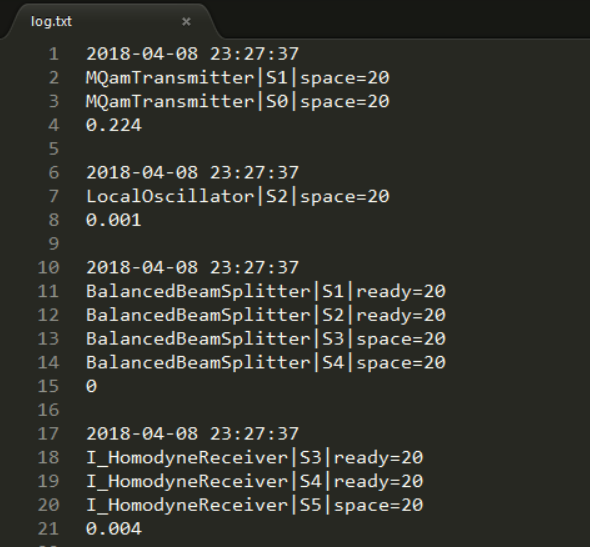
\includegraphics[width=.35\linewidth]{./chapter/simulator_structure/figures/output_file}
\caption{Output File Example}
\label{fig:outputfile}
\end{figure}

Figure \ref{fig:homodynesignals} shows a portion of code that consists in the declaration and inicialization of the I\_HomodyneReceiver block. In line 97, we can see that the block has 2 input signals, $S3$ and $S4$, and is assigned 1 output signal, $S5$. Going back to Figure \ref{fig:outputfile} we can observe that $S3$ and $S4$ have 20 samples ready to be processed and the buffer of $S5$ is empty.

\renewcommand{\figurename}{Figure}
\begin{figure}[H]
\centering
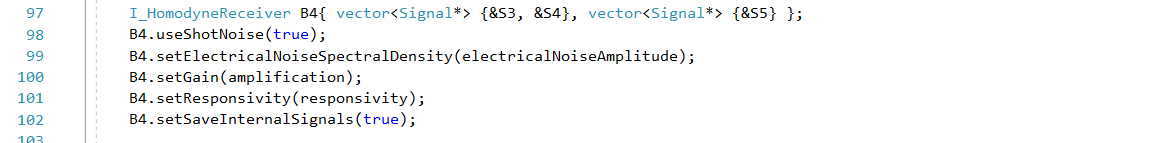
\includegraphics[width=1.3\linewidth]{./chapter/simulator_structure/figures/homodyne_signals}
\caption{I-Homodyne Receiver Block Declaration}
\label{fig:homodynesignals}
\end{figure}

\subsection{Testing Log File}
In directory \textit{doc/tex/chapter/simulator\_structure/test\_log\_file/bpsk\_system/} there is a copy of the BPSK system. You may use it to test the Log File. The main method is located in file \textit{bpsk\_system\_sdf.cpp}

% bibliographic references for the section ----------------------------
\clearpage
\printbibliography[heading=subbibliography]
\end{refsection}
\addcontentsline{toc}{subsection}{Bibliography}
\cleardoublepage
% ---------------------------------------------------------------------


